% !TeX root = ../main.tex
% Add the above to each chapter to make compiling the PDF easier in some editors.

\chapter{Performance and Evaluation}\label{chapter:evaluation}
\section{Field Test}
To deploy our project in the field, we used IBM Cloud's free hosting service to run our node.js server and connect it to our MongoDB, as mentioned earlier Atlas instance. We tested the system over the course of eight days from Wednesday, the 29.01.20 to Wednesday, the 05.02.20. To find participants, we asked friends, acquaintances. We tried to recruit people in the vicinity and over private social media channels. Still, unfortunately, because of privacy concerns, we only found 13 volunteers to participate in the trial, of which only 5 to 7 devices were available over the whole test period. Because of Android's own battery management system and other OEM's aggressive battery saving algorithms, a lot of devices were not reachable after they have been unused for a longer period of time, entering Doze mode. Additionally, most of our users were fragmented globally, and with the low number of active participating devices, we had to adapt our aggregation parameters. To start aggregation processes, we use Postman, a tool for sending among others REST requests directly to an address.
% Todo: \cite[Postman]

We started with aggregating similar data to Simon van Endern, such as steps data and activities data, and afterward, we looked into location data and presence data. The collected data set can be found in the Git repository [X] and partially in the sections below.
% Todo: \cite[Git repository] upload JSON
\subsection{Data Consumption}
Running the application by itself shouldn't require a lot of data, as the only data consumption only comes from the initial registration request to the server, the periodical ping to the push service, and the aggregation requests. We let the application run for the first few days and aggregated data irregularly starting after the 29.01.20. But most of the requests were sent towards the end of the field test, on the 05.02.20 and the 06.02.20. In the figure \ref{fig:diagram_requests}, the distribution of the aggregation can be seen. We were able to request proof of data consumption from 4 participants, but are only able to confirm that some of them were actively providing data in requests. The provided screenshots can be viewed in the Appendix, and consumption is shown in table [X]. 

\begin{figure}[htpb]
  \centering
  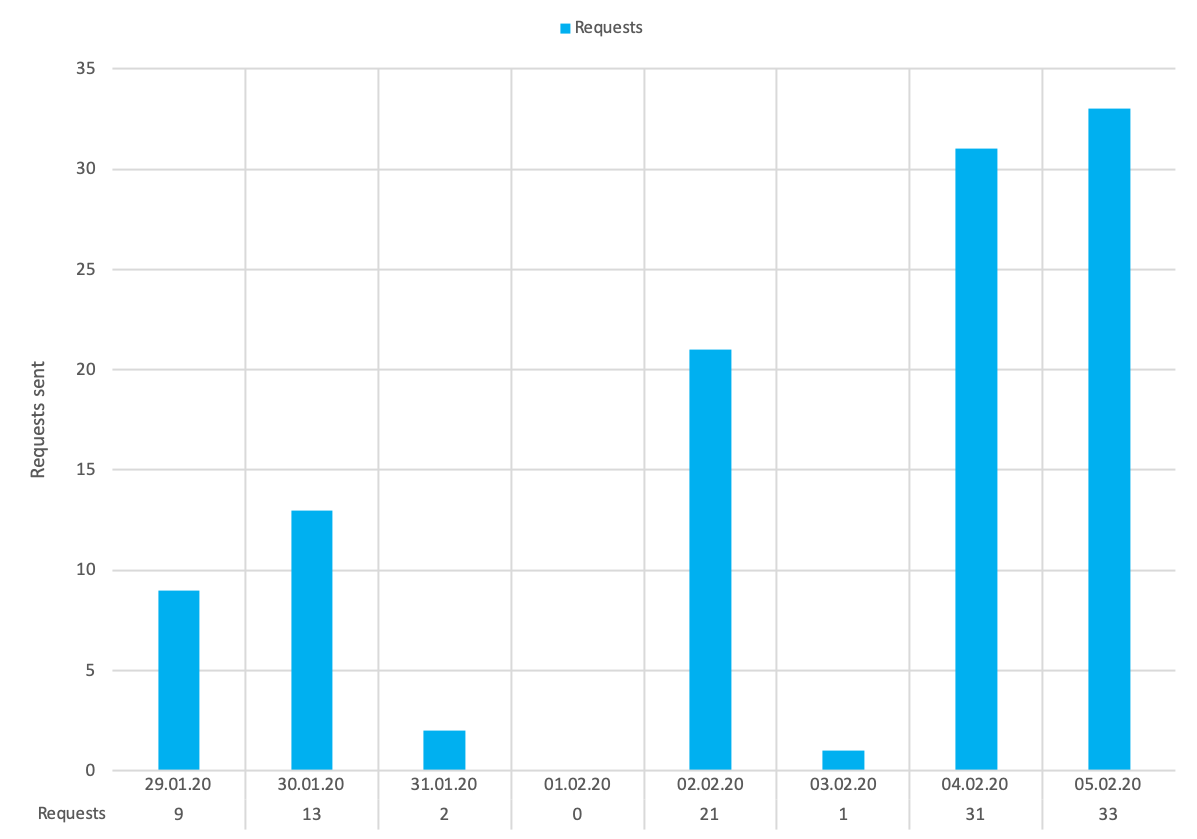
\includegraphics[width=0.8\textwidth]{figures/diagram_requests.png}
  \caption{Simon van Endern's original architecture.} \label{fig:diagram_requests}
\end{figure}

% Todo: insert table for request distribution
% Todo: insert table for data consumption
We can see in all cases that data consumption didn't exceed 10MB and, in most cases, didn't even use more than 5MB. We could extrapolate that the consumption of data should not be a lot more than twice, depending on the number of aggregation requests sent because the parallelization of the data collection should always aim for small groups.

\subsection{Results}
We sent more than a hundred aggregation requests during the field test. We collected the average number of steps taken and the average time spent on the activities still, walking, biking, and in a vehicle. The start and end date parameters for aggregating these types were to 12:00 am JST for each day. We also requested for location and presence of the devices over the globe at 12:00 pm CET and 12:00 pm JST, 11:00 am, and 3:00 am in the GMT zone, respectively. Each aggregation had consistently from 3 to 7 participants.

% Todo: insert figure
% Todo: describe all the data collected and add figures
% Todo: inconsistency because of the epoch time difference

We recorded the average time spent motionless was from 577 to around 1106 minutes. For individual participants, we have a wide gap with a minimum of 0 and a maximum of 1310 minutes, almost 22 hours, spent still, as depicted in figure \ref{fig:diagram_still}. This can be explained on the basis that for counting activities, we only use finished activities that have a start and an end timestamp. For the two cases, it was highly probable that the phone hasn't been used touched for two full days, and thus the start date of the activity was before the 31.01.20 and the end after the 01.02.20. For the low values of 16 minutes and 28 minutes, we have not found an explanation. 

\begin{figure}[htpb]
  \centering
  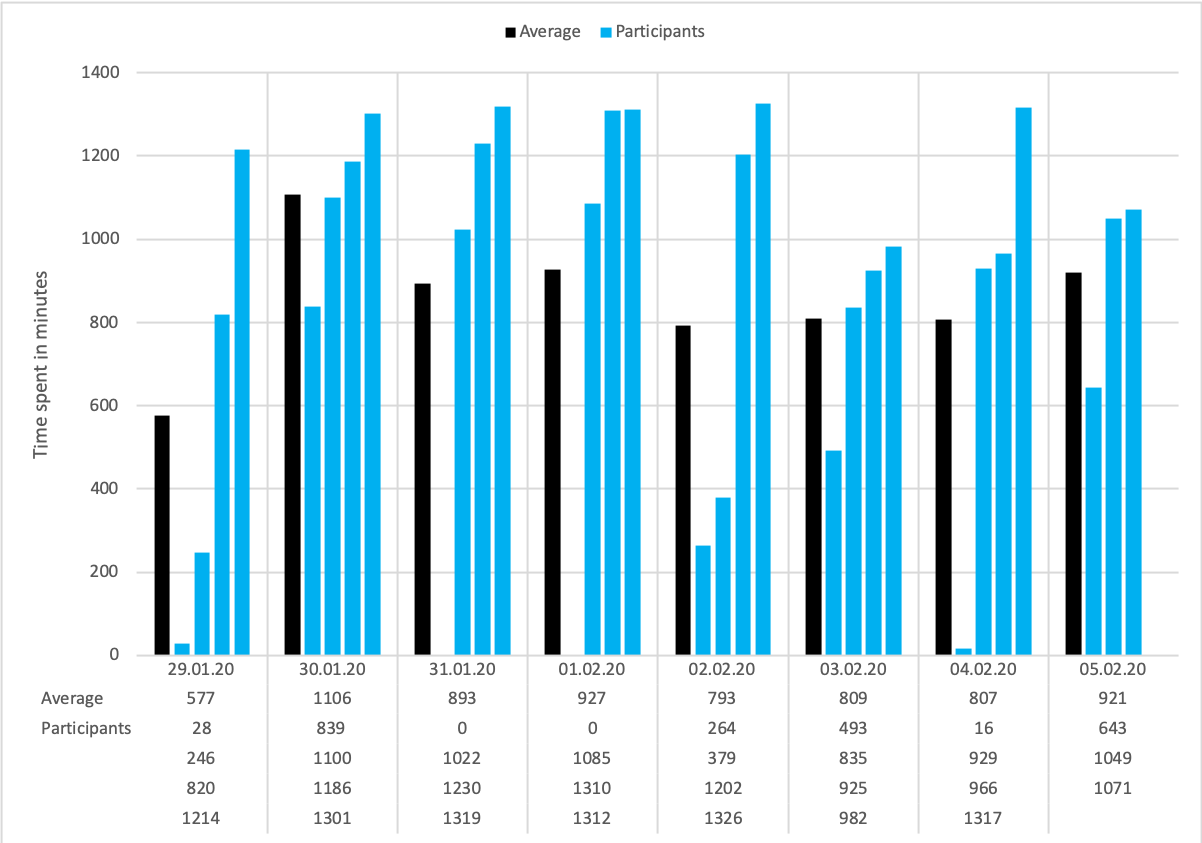
\includegraphics[width=0.8\textwidth]{figures/diagram_still.png}
  \caption{Distribution of still raw values.} \label{fig:diagram_still}
\end{figure}

As for walking, figure \ref{fig:Diagram_Walking} shows a mean time between 25 and 75 minutes, from participants only walking 2 minutes up to 158 minutes. Without having the running time at hand, it is possible to infer that with the high number of steps recorded on half of the days, that one person is running regularly if the steps can be assigned to the same user.

\begin{figure}[htpb]
  \centering
  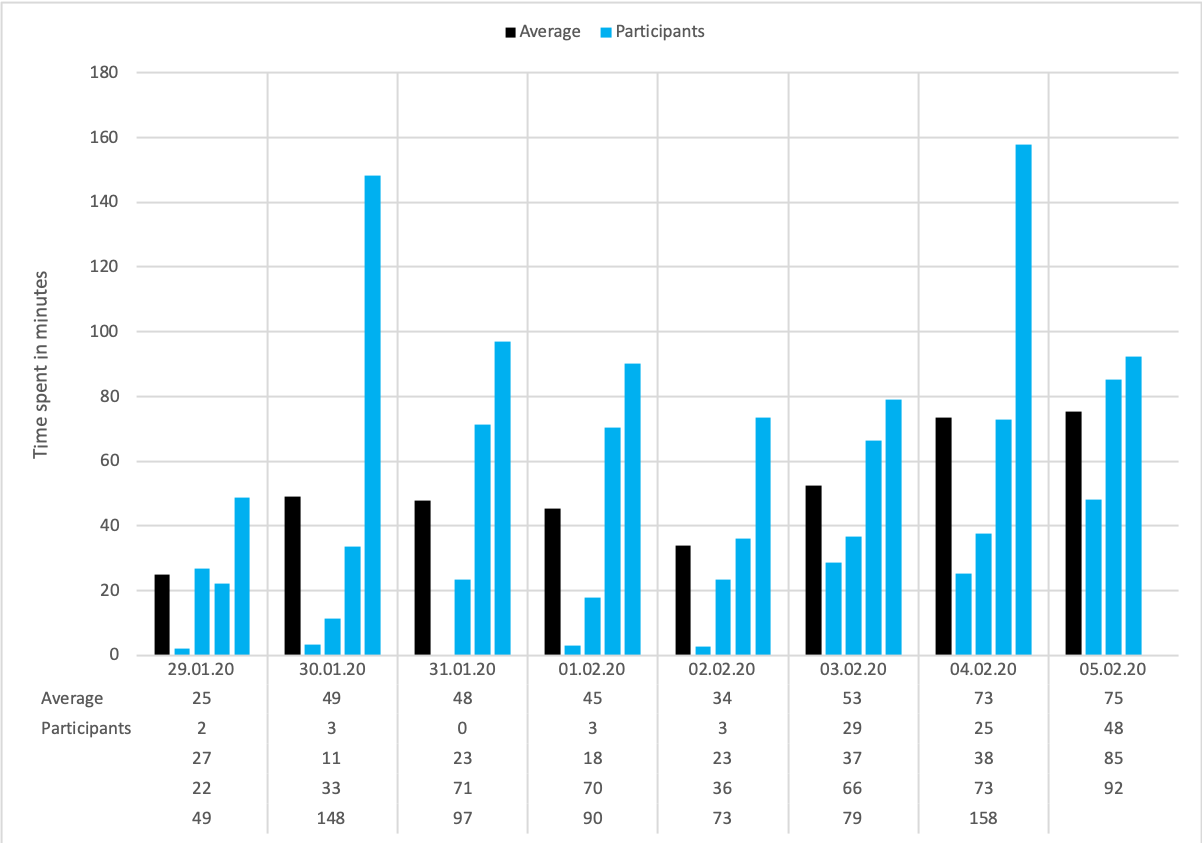
\includegraphics[width=0.8\textwidth]{figures/diagram_walking.png}
  \caption{Distribution of walking raw values.} \label{fig:diagram_walking}
\end{figure}

On average, the participant uses a vehicle for up to 106 minutes. On occasion, many users don't use any transportation at all. Figure \ref{fig:Diagram_Vehicle} shows the data a user spent in a vehicle. Registered activities from 1 to 2 minutes are with high probability credited to escalators and elevators.  

\begin{figure}[htpb]
  \centering
  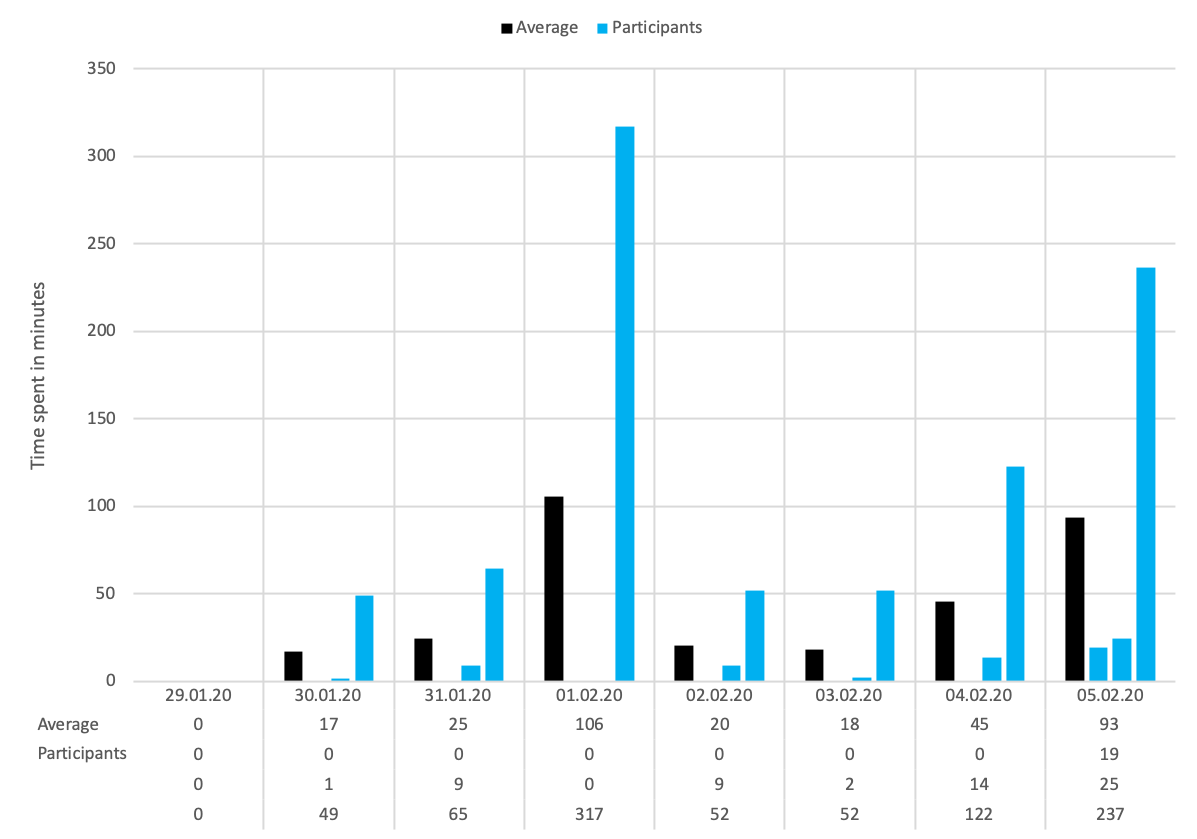
\includegraphics[width=0.8\textwidth]{figures/diagram_vehicle.png}
  \caption{Distribution of in vehicle raw values.} \label{fig:diagram_vehicle}
\end{figure}

For cycling, on some days, we only had one value of around 7 minutes. We can assume with confidence that it is one specific participant that is using the bike on occasion.

% Todo: write about the location data
Now we take a look at the location and presence data. In the tables [X] and [X], we can see the GPS coordinates that we get after the server suppresses them for k-anonymity. We do this because there is a lot of information if only one person in a greater area is present. If we collect only spatially cloaked area in the vicinity and we do this for several time points, we can assume with high confidence, the general trajectory of that user posing a risk to privacy.
% Todo: insert table

According to the aggregated data, we have 2 to 7 participants throughout the field test. Table [X] shows the location at 12 pm JST and table [X] at 12 pm CET, which corresponds to 4 am CET and 8 pm JST in the other time zone. As already mentioned before, because of the fragmented participant pool, we set the desired location at any GPS coordinates. Still, the range to 50,000km and the accuracy to 0, which results in gives us a rough estimate in a 111km range [X].
% Todo: \cite[GPS accuracy] 

At 12 pm JST or 4 am CET, we have only two devices located in the greater Munich area with a midpoint of \((48.50108260577674, 11.495067909974292)\) which corresponds to the territory covered by \(\langle(48, 11),(49, 12)\rangle\). On the 30th and 31st of January, we detected three devices in the same region and, additionally, 2 participants close to \((35.50103138028429, 139.49688751384306)\) which represents the space between \(\langle(35, 139),(36, 140)\rangle\). For the rest of the field test, we can determine two devices in the general area of Munich and 2 in Tokyo most of the time.

As for the aggregation at 12 pm CET or 8 pm JST, we get similar results with three devices in the greater Munich area and also three devices in the proximity of Tokyo for four days. On the 30.01.20, we only see 2 users the area covered by \(\langle(35, 139),(36, 140)\rangle\) and on the 05.02.20, we only see 2 users between \(\langle(48, 11),(49, 12)\rangle\).

Figure \ref{fig:acc0} depicts the areas that are spanned by the corner points for Munich and Tokyo. 

\begin{figure}[!tbp]
  \centering
  \subfloat[Munich][Munich \(\langle(48, 11),(49, 12)\rangle\)]{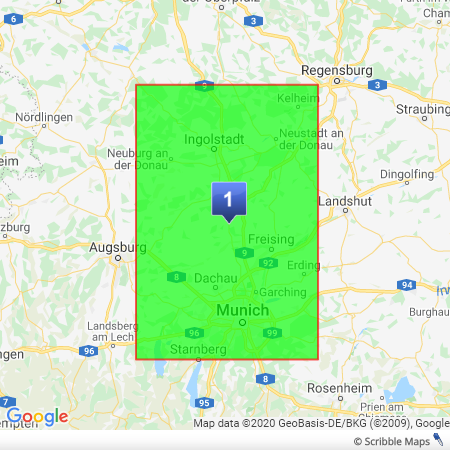
\includegraphics[width=0.45\textwidth]{figures/acc0_m}\label{fig:acc0_m}}
  \hfill
  \subfloat[Tokyo][Tokyo \(\langle(35, 139),(36, 140)\rangle\)]{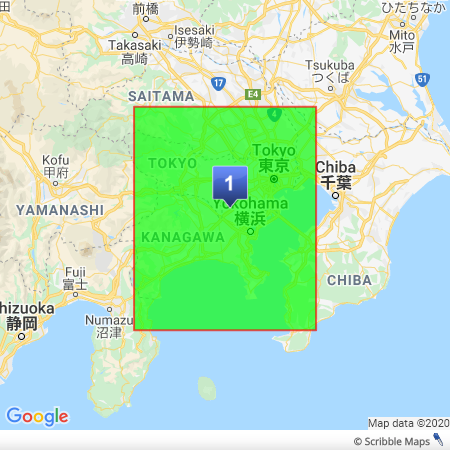
\includegraphics[width=0.45\textwidth]{figures/acc0_t}\label{fig:acc0_t}}
  \caption{Spatial areas in Tokyo and Munich with an Accuracy of 0}
  \label{fig:acc0}
\end{figure}


\subsection{Privacy Evaluation}
After collecting the data, we analyze it for privacy issues. We first put the steps data and activity data under the microscope, and then we tear down the location and presence information. Examining possible reconstruction, linking, or tracing attacks.

\subsubsection{Raw Values of Steps and Activities}
Looking at the steps and the activities, we don't see any vulnerability in linking attacks as there are not a lot of possible quasi-identifiers to connect. Being able to connect temporal similarities would be a potential vulnerability. Steps data is collected over the course of the whole day, but could also be modified to use a specific time frame instead. But the issue is, that all delivered data from every device has the same time data they get from the request. The same applies to activities. As every query by itself is a statistical database, without any quasi-identifiers, it is improbable to achieve a linking attack. 
Tracing attacks, however, can be used to identify if a user is used in the query, possibly. Taking the gathered steps data, with auxiliary data as knowing the exact number of steps a person took, we can infer that the person has participated in the aggregation request with a high chance. But because our data collection architecture has a possibility that a person doesn't provide data, there is plausible deniability. Scaling the number of participants up, would result in a normal distribution of the mobility data, as shown by T. Althoff et al. With a lot of possible users, inferring the participation of one user, even with the ability to match the number of steps to exactly one value in the query result, we are unable to guarantee the user took part. We think we can assure privacy with the raw values, the same as Simon van Endern promised privacy for median values.
% Todo: \cite[Large-scale physical activity data reveal worldwide activity inequality]

\subsubsection{Location and Presence}

As for the more specific mobility data, we can't build any connections to the other data with confidence. We are incapable of linking our location or presence to steps or activities without auxiliary data. By suppressing unique locations, that could show individuals, and we have a k-anonymous data set. But the same problems apply to it as for steps and activities. Missing quasi-identifiers make it hard to re-identify the devices that the data came from. 
But in contrast to reconstruction or linking attacks, tracing attacks could be used. Because of the lack of participating devices, we are sure that it is the same people participating in the query. But with the low accuracy, we are unable to build any trajectories. To examine the possible calculation of paths, we need more data and more accurate data.

\section{Simulated Test}
Because of the small sample size in our field test, we decided to run one more test in a more controlled environment for more reliable data. We use 10 Android Emulators on different versions of the operating system using Android Studio. We selected four small landmarks in a small area from which the devices travel from one of the other landmarks as a destination. This will ensure that we have devices that have been alone and together over the test period. For 10 minutes, each device generates location data along a predefined route in an interval of one second, totaling in 600 GPS coordinates. We use the emulator's route simulation, which leverages Google's Map API, giving us a travel speed of exactly 4.5km/h. We then aggregate the location data over the ten minutes for each minute and gather data using different accuracy parameters, giving us different approximate areas. This gives us more data to evaluate privacy issues, especially concerning historical location data.

\subsection{Results}
First, we chose an accuracy of 2 decimal places, which translates to real-world distances of around one kilometer. We were able to track 7-8 devices consistently in the areas depicted in figure \ref{fig:acc2}. The markers 1 and 2 span the area of \(\langle(35.54, 139.63),(35.55, 139.64)\rangle\) and the other two markers are \(\langle(35.53, 139.63),(35.54, 139.64)\rangle\). Table [X] shows how many devices were in which area at each time step. 
% Todo: insert table

\begin{figure}[htpb]
  \centering
  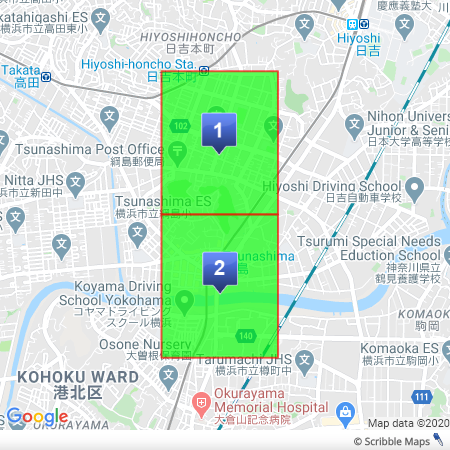
\includegraphics[width=0.5\textwidth]{figures/acc2}
  \caption{Distribution of still raw values.} \label{fig:acc2}
\end{figure}

Because the region we specified is large, we can almost always find multiple devices in the area.

\begin{figure}[htpb]
  \centering
  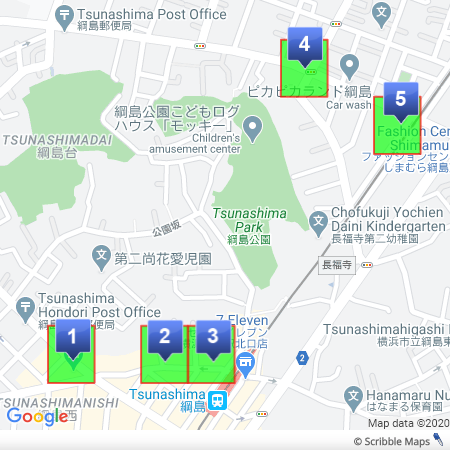
\includegraphics[width=0.5\textwidth]{figures/acc3}
  \caption{Distribution of still raw values.} \label{fig:acc3}
\end{figure}

For our next aggregation, we selected a precision of 3, which corresponds to roughly 100 meters. The data in table [X] reveals that we can find two mobile phones most of the time, with aggregations, in which we were able to find three devices or none at all. The areas are visible in figure \ref{fig:acc3}.

Finally, we send requests with an accuracy of 4 or 10 meters. In this scenario, we were almost unable to register any devices, except for minute 10. At this time point, we have two users that pass each other in \(\langle(35.5372, 139.6336),(35.5373, 139.6337)\rangle\) as seen in figure \ref{fig:acc4}.

\begin{figure}[htpb]
  \centering
  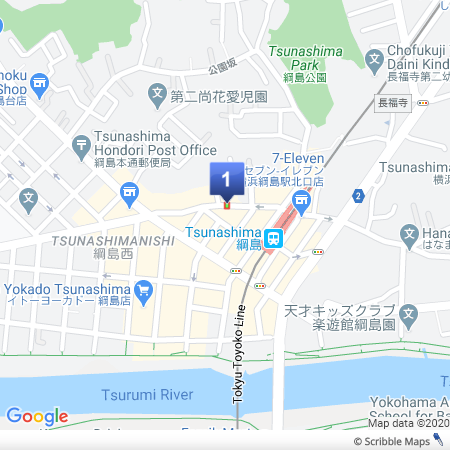
\includegraphics[width=0.5\textwidth]{figures/acc4}
  \caption{Distribution of still raw values.} \label{fig:acc4}
\end{figure}

\subsection{Privacy Evaluation}
Looking at the documented results, we can see where devices meet each other. With low precision, we always register 3-4 users. Using k-anonymity, we are unable to find out more than the provided data. We only know the number of people present in a specific area. 

After we increased precision to 3, we mostly see pairs. According to the table [X], in the first 3 minutes, we can assume that two devices pass each other in the same area. Later one of them leaves the zone, and we stop registering that region. Without auxiliary information, we are unable to find out in which direction the users traveled or who left the area first. In minute 5 to 9, we register two adjacent regions. We can assume that there are more than two phones in the vicinity. Analyzing the historical spatial data, we suggest that we have two devices in area 2 and one device in zone 3 at minute 5. In the sixth minute, we register a new domain and loose the old one, indicating that one device moved from region 2 to 3 while the other two are still in their respective areas. In minute 9, we then see the old area again and the new one vanishing, suggesting that the device that was formerly in area 3 walked into zone 2. We were able to infer the travel direction of one device, but are still unable to point out the device.

Using an accuracy of 10 meters, we are unable to collect any useful data with the lack of devices.

\subsection{Usability}
By stripping away all of the quasi-identifiers, we sacrifice a lot of possible usability in the data. But for the loss of value, we are able to preserve a lot of privacy and even provide anonymity. On the one hand, we won't be able to use the collected data for detailed medical research that requires sex, age, and other information. On the other hand, however, we can gather population density data and activity data, which are very handy in urban planning. This provides a good starting point to find a balance between the usability of data and the privacy of the data provider.

\subsection{Possible Improvements}
We achieved a lot of scalability and a lot of privacy in our implementation, but there are still immediate improvements possible in both the application and the server. For the spatially cloaked location data, our design only applies static accuracy provided by the request itself. It may be possible to send different accuracies of the concealed areas and match them on the server, to get smaller anonymizing regions and, at the same time, still maintain k-anonymity.

The application should also be tweaked to be able to handle multiple requests at the same time. It is thus making data aggregation, in general, more efficient. The same applies to the server. At the moment, it doesn't differentiate the messages it receives from the groups. It is forcing researchers to wait for an aggregation to finish before they are able to send a new request.

As homomorphic encryption is still in its infancy, an alternative to protect the first participants from the subsequent is to add dummy data that can be removed at the end. This method would hide the primary data added to the aggregation and make it harder for the second device in the chain to determine the real input from the fake.

We also have an issue with the confirmation approach. This method is right now implemented using a sleeping thread that prepares to resend the data collected so far to the subsequent device after time out, but which in turn creates another sleeping thread. It may lead to multiple threads that use a lot of resources and might cause the application to freeze or crash.

